%%%%%%%%%%%%%%%%%%%%%%%%% start of article main body
% <put your article body there>

%%%%%%%%%%%%%%%%
%% Background %%
%%
\section{Introduction}
%Mobile network simulations are used to evaluate the behavior of mobile radio networks under different scenarios. One of such scenarios is the mobility simulation. Hereby, mobile subscribers move freely in the research area. Throughout their travel, their mobile station connects to different cell sites. The movement can also be seen as a transition of network load. When a mobile subscriber leaves to work, the network load transitions with them. To investigate the effect of moving subscribers; the subscribers mobility needs to be predicted.  Typical mobility simulations are either done by creating network load maps or by using stochastically functions to describe the mobility behavior. 
%
%Our approach utilizes handover events. Consecutive Handovers during a call will be combined to a handover sequence. This sequence will be used to model the subscriber mobility. Handovers are essential for a cellular network since they allow the subscriber to move from the coverage area of one cell site to another while still maintaining an ongoing call or data transfer. By estimating the origin of each handover event a trajectory can be computed. The computed trajectory represents the subscriber route. The time of occurrence of a handover event is used as the timestamp. Timestamps in combination with the traveled route will later be used to compute the average velocity for each route segment between two consecutive handover events. Thus, the system can only compute the average velocity for each route segment; the smaller the coverage area of succeeding handovers is, the more accurate the velocity will be. The main limitation of our approach is that it only works for subscriber in connected mode. Therefore, it can only be used to generate trajectories for subscribers during a call. However, this limitation is not a drawback for network simulation since most of the traffic is produced by connected subscribers.
%
%This approach allows mobile network operators to test their mobile networks with simulations based on their own subscriber behavior. The benefit is that trajectories can be generated for each particular time. Therefore, this approach can be used to investigate, how changes in the network infrastructure deal with recent scenarios.  Annotating the derived route with timing information is an important figure as it influences the network load and traffic. 
%
%The aim of this research work is to produce trajectories that can be used for mobility simulations in mobile networks. It allows network operators to test their networks with data derived from their subscribers. 


At this time, there are in general two types of mobile networks simulations in use. The first ones are applied during the design and development stage of the mobile network. These simulations are used to test individual parts, sub systems or the whole network. They are usually done when a new standard for a mobile network is defined or when new parts are developed. On the other hand, the second kind of simulations focus on the operation of the network. They are used to investigate how the subscriber's behavior affects the mobile network. The investigations can either be done in a virtual network to develop and test new algorithms and approaches or in a real network to test it under certain scenarios. Both, the virtual and the real network simulations require moving subscribers in the research area.

Therefore, our research focuses on a real network simulations and how to estimate the subscriber's mobility. Thus, the simulations needs information about the environment (cell site location, soil conditions, and elevation profiles) and the subscriber's mobility. The mobility can either be derived from a stochastic process or from real subscriber's behavior. In our work we are using events captured in a core network to estimate the mobility of real subscribers in the network. Finally, we analyze handover events in order to estimate the subscriber's route and its velocity.
The Austrian network operator A1, provided us with data of active (connected-mode) GSM speech subscribers. This is due to the fact, that only active subscriber's issue handover events. However, the framework can also work with idle subscriber and data (2G, 3G and 4G) subscribers for which location area updates exist, instead of handover updates. In our work we focus on handover events, since these events have a better location accuracy.
Another part of our work is to model the real network as good as possible, with freely available datasets, since mobile network operator are not wiling to share these datasets with third parties. These datasets contains the BTSs configuration, antenna characteristics, antenna tilt, etc. We are investigating how well a mobile network can be modeled without having to rely on the network operator itself.
We found out that, despite the fact that we are using freely available datasets, trajectories can be estimated for urban, as well as semi-rural areas. Our approach can also estimate the velocity of the subscriber's on the road network and is therefore well-suited to describe its mobility.

\section{Related Work}
Over the past years research has been conducted in the field of mobility simulations and investigation of mobility related events in mobile communication networks. Besides mobility simulations and mobility modeling, mobile subscription data is also used for travel time estimation in ITS applications. We summarized fundamental concepts in both mobility simulations and travel time estimations.
\paragraph{Mobility Simulations}
To simulate the mobility in mobile communication networks, stochastic processes are used. The mobility behavior of subscribers is modeled as a stochastic process. The most common mobility models are random way point (RWP) or random walk models such as Brownian motion (BM)~\cite{Klafter1996} , Levy walks and flights~\cite{Camp2002}, and also the Markov mobility\cite{Bai2004}.
Rhee et al.~\cite{Rhee2011} compared the Levy walk model, which is an extended random walk, with the human mobility. GPS traces of 101 volunteers were used to compute the similarity. Their findings indicated that outdoor Levy walks with less than 10 km contain statically similar features to the human walk.
To understand human mobility patterns Marta C. Gonzalez et al.~\cite{Gonzalez2008} analyzed 100000 anonymized trajectories of mobile subscribers. They found out that human mobility is characterized by a time-independent travel distance and that they travel to a few highly frequented locations. However, this result were only used to evaluate the mobility of many and not single individuals.
\paragraph{Travel Time Estimation}
The following research is based on passive tracking. Passive tracking uses mobile subscriber's events captured in the core network to locate the subscriber. Therefore, passive tracking does not require any equipment in the mobile station or involvement of the mobile subscriber. On the other hand, active tracking requires the participation of the mobile subscriber and the mobile station. Active tracking technologies are Global Positioning System (GPS) and Time Difference of Arrival (TDOA). Systems like TDOA need BTSs that support that feature and therefore require special equipment. These systems have a higher location accuracy than passive tracking system, but they increase either the power consumption of the mobile station (GPS) or the network load (TDOA) or both.\newline

Martin Alger~\cite{Alger2004}, from Vodafone Germany, was one of the first who investigated travel time estimation on the German higher roads network. Double handover (DHO) events were used to compute the cell drive through time, which is the time between entering the cell coverage and leaving it. By estimating the route a subscriber drove within the cell coverage and dividing it by the time difference, the velocity could be computed. An average filter was used that combined the travel times of other subscribers in the same cell to remove stale information. The system was used to investigate the traffic condition on the higher roads network in real time. Their research showed that travel times can be estimated for the higher roads network without the need of expensive inductive loop detectors. However, their approach focus only on the highway networks and does not support the minor roads network. The German road network\footnote{Statistic about the German roads network January 1, 2013 \url{http://www.statistik-portal.de/statistik-portal/de_jb16_jahrtab36.asp}} consists of $12.879$km highway and $230.517$km other roads and therefore their approach is only applicable for $5.59\%$ of the total road network.\newline

To measure the traffic velocity and travel time in Israel, Bar-Gera~\cite{Bar2007} used a proprietary system by Estimotion Ltd. This system works with handover events to derive the traveled route and velocity. A sequence of locations derived from the handover footprint is matched to road segments. The length of the road segments together with the estimated handover position was used to derive velocity information. The eEstimated segment velocity of individual drivers was later combined with velocities from other drivers on the same segment to increase the accuracy and remove noise.

\paragraph{Contribution}
Our goal is to estimate movement trajectories for cellular network subscribers with a combination of closed and public available datasets. The developed framework allows transforming subscriber's information form a network operator into trajectories of subscribers. Our approach works passively and does not need any participation of the subscriber's. Therefore, we can estimate trajectories for each subscriber in the network.

As well as that, we are evaluating how the coverage area for cell sites of a real network can be estimate with limited information. This is different to most research projects~\cite{Gonzalez2008,Tettamanti2012} since they are relying on Voronoi diagrams. Part of this research was to evaluate the accuracy of Voronoi diagrams and coverage predictions done with a network planning tool.

Contrary to Bar-Gera~\cite{Bar2007} and Alger~\cite{Alger2004} we are estimating trajectories for individual subscribers and are not combining them. Additionally our approach works also for the minor roads network unlike the system developed by Vodafone.

In contrast to others, our trajectories are time-dependent and can therefore react to seasonal changes or different weekdays. This is important since the behavior of the subscriber will be different for example during workdays and weekends or between summer and winter.

Another benefit is that previous incidents in the network can be replayed and simulated by generating trajectories for the particular day with our framework.

%We estimate trajectories for mobile operators based on mobile subscription data. These trajectories cover the whole route a subscriber drove during an active call. The trajectories will consist of the route and an approximated velocity derived from handover events. We investigated how the location of handovers can be computed. Since our system requires the coverage area for cell cites we evaluate two different approaches tow estimate the coverage area for a given network.
%We want to enable network operators to simulate their real network or a virtual network with driving trajectories of their own subscribers.

\section{Methodology}

In this section, we introduce our approach about how to estimate movement trajectories for cellular network subscribers. At first, we are introducing the dataset we are using and additionally, data sources which we require for the operation of our framework. Followed by a delineation of our approach and the algorithms used to transform the input data into estimated movement trajectories. We describe how the start and end point of a trajectory and its route can be predicted and how to derive the subscribers velocity from handover events. At last, we present how the validation of the approaches was done. We introduce the metrics used to evaluate the different aspects of the trajectory estimation such as handover position, route geometry and velocity. 

%In this section, we introduce the dataset and the approaches used to estimate movement trajectories for cellular network subscribers. Our approach uses handover updates in combination with cell area estimations to estimate the users' movement over time. This approach allows network operators to analyze their networks with real subscriber mobility simulations. A limitation of this approach, however, is that it can only estimate trajectories for active subscribers (during a call). Since only active subscribers are participating in the network this is not a drawback for mobility simulations.

\subsection{Dataset}
The trajectory estimation process utilizes different types of data in order to derive the subscribers mobility. At first, we are introducing the dataset provided by the network operator. This dataset consists of subscriber's information (call establishment/termination, handover) and the location of each cell site. Since GSM does not directly expose the subscriber's location, only the current cell site is known. Therefore, we need additional data sources to enhance the positioning. These data sources are used to estimate the border of each cell site, they help to predict the start and the end position of the trajectory and to derive the subscriber's velocity.
\subsubsection{Provided Information}
In order to estimate the subscriber's mobility we need a record of its behavior. The subscriber's behavior can be derived by capturing events in the networks operator's core network. The process of capturing subscriber's events by installing network probes into the core network is described by Valerio~\cite{RoadCell2009}. From the subscriber information we can derive a coarse location of the subscriber by simply looking at the Cell-Id and Location Area Code (LAC). Together with the timestamp of the event, the mobility can be derived.

An event captured in the core network consists of the following attributes:
\begin{itemize}
	\item Time stamp, time when the event was captured
	\item Id, identifies the subscriber
	\item Cell-id, id of the currently connected cell id
	\item LAC, location area of the current cell
	\item Event, defines the captured event
\end{itemize}

An example for events captured in the core network is depicted in Table~\ref{table:events}. Here the first event describes a call establishment, followed by three handover events and at last, a call termination event. \newline
\begin{table}[h]
		\caption{Events captured in the core network of the network operator}
		\begin{tabular}{|c|c|c|c|c|}
			\hline
			Time stamp & Id & Cell-Id & LAC  & Event              \\ \hline
			1327678833 & 4  & 51520   & 5501 & Call Establishment \\
			1327678854 & 4  & 31510   & 5501 & Handover Update    \\
			1327678935 & 4  & 31210   & 5502 & Handover Update    \\
			1327678949 & 4  & 40510   & 5502 & Handover Update    \\
			1327679027 & 4  & 40510   & 5502 & Call Termination   \\ \hline
		\end{tabular}
		\label{table:events}
\end{table}

%This data was later used to produce handover sequences. The later transformed handover sequences have the same format as the handover sequences captured in a network operator core network (see Table \ref{table:transformed}).
%
%The GPS position is used to validate our results, in terms of route geometry and estimated velocity. An important aspect of using GPS is that besides the route geometry it also reveals the exact location of the handover. Thus it enables us to evaluate the accuracy of the handover position prediction. Besides the actual traveled route, the GPS information together with the time stamps allows deriving the actual velocity of the driver. Therefore, GPS is used to measure the difference between the estimated velocity and actual subscribers' velocity.
%
%The GPS information is only used for validation purposes as it is not available later, due to the fact that the event capturing takes place in the operators core network instead of in the handset.
%
%During our research, handover sequences were captured for both semi-rural areas and urban areas. The research area covers roads of the higher road network as well as of the minor road network. The urban research areas are within the city of Linz and Vienna in Austria. The semi-rural  research area is between the city of Linz and the town Hagenberg in Mühlkreis.

The second data, which was provided by the network operator, was the location of its cell sites. This dataset consists of the cell tower location, specified by the latitude and longitude coordinates, and an angle, which defines the main beam direction of the transmitter. However, many base transceiver stations (BTS) will share the same location, as only the location of the tower for each BTS is known.

\subsubsection{Additionally Data Sources}
For now we know the subscribers behavior over time by investigating the events in the event stream and the location of each cell site. However, this data is not sufficient to estimate the movement trajectory for the driver. Therefore, the framework needs additional data sources that will be introduced in this section.

\paragraph{Cell Area Estimation}
As of now, we only know a coarse location of the subscriber, defined by the location of the currently connected cell site. An important aspect for the estimation of the movement trajectory is the subscribers' location. Since the only information that is available is the currently connected cell site, an approximation of the cell sites coverage area is needed. The coverage area for the currently connected cell site narrows down the subscriber's location, as it is in general implausible that a subscriber is located outside the coverage area of the cell site. We are investigating two different types of cell area estimation. The first, Voronoi diagrams, are using the location of all cell sites and defining a polygon for each cell site. A subscriber located within this polygon has the closest distance to the cell cite, to which the polygon belongs. The second, coverage prediction, is using a network planning tool and besides taking the location of the cell sites is also taking the environment into account. The environment is defined as the elevation of the surface, the transmit power, etc. \newline


A simple approximation of the cell area can be derived from Voronoi diagrams as described by Baert and Seme~\cite{Baert2004}. Hereby, Voronoi tessellation, is used to partition a plane with $n$ points into $n$ convex polygons~\cite{Aurenhammer1991}. Each of this convex polygons contains one generator point, which in our case the location of the cell sites are. %which in our case are the locations of the cell sites. 

However, many of the cell sites consists of more than one BTS and form a sector antenna. Since all of these BTS have the same location, their coverage area would be identical.

We overcome this by moving the location of each sector, based on the angle of the sector, out of the center location of the cell site. The longitude's location of the sector will be moved with Equation~\ref{eq:sectorX} and likewise the latitude's location will be moved with Equation~\ref{eq:sectorY}. The constant factor $\frac{1}{50000}$ means a maximum movement of $1.6$ meters in either direction.

\begin{align}
	x & =x+\cos(\alpha)\frac{1}{50000}\label{eq:sectorX}  \\
	y & =y+\sin(\alpha)\frac{1}{50000} \label{eq:sectorY} 
\end{align}
\newline

A more accurate method for estimating the coverage area is the use of a network planning tool. Voronoi diagrams only use the location of each cell site, however, in a real mobile network the coverage area is influenced by a variety of factors such as:
\begin{itemize}
	\item Network load
	\item Antenna characteristics
	\item Transmitter power
	\item Shadowing
	\item Landscape characteristics
	\item Surrounding cell cites
\end{itemize}

We estimated the coverage area for all cell sites of the Austrian network operator A1 in the research area. The accuracy of the coverage prediction depends on the quality of the input data. Since A1 only provided us with the location and the beam direction angle of its antennas, we were using publicly available datasets, to enrich our coverage estimation. Part of these datasets are digital elevation models, building models and a transmitters power database, that will be used by the network planning tool for the coverage prediction.

\paragraph{Estimation of The Transmitter Power}
The coverage area directly depends on the transmitter power of the antenna. We are using transmitter power measurements from the Austrian Forum Mobilkommunikation (FMK) to enhance our coverage prediction. The FMK provides a service, where participating mobile network operators can upload information about their infrastructure. Most important for our work was the location and measurements of the transmitter power of cell sites.

However, there are a few limitations while using this data. First, the service provided by the FMK is voluntary and therefore the data can either be out of date or absent. Second, only the highest transmitting power of all sectors located at the same cell tower is provided. Last, there is no information available to which network operator the cell site belongs to.

In the following paragraph the approach to retrieve transmitter power estimations for each cell site is described. At first we define two sets, one for the cell site locations of the provider and one for the FMK transmitters.
Let $A=\left\lbrace pos_0,pos_1,...,pos_i \right\rbrace $ be a set of cell site location of the networks operator and $B=\left\lbrace pos_0,pos_1,...,pos_j \right\rbrace$ be a set of cell site locations provided by the FMK. From these two sets we can then derive an intersection $C=A \cap B$ of cell site locations that are present in both sets. Additionally the set $C$ contains the transmitter power for each cell site from the FMK set $B$. The intersection performs a filter process and ensures that only cell site locations from the FMK are used which belong to the networks operator. To estimate the transmitter power of cell sites not contained in $C$ but  contained in $A$, a scattered interpolation is performed. The scattered interpolation process takes the location and the transmitter power of the set $C$ and interpolates the transmitter power for the set $D=A \backslash B$.
An example for a scattered interpolation done for 20 random cell site with a random transmit power in the range of 45-52dBm is depicted in Figure~\ref{fig:transmitpower}.
	\begin{figure}[h!]
		\label{fig:transmitpower}
		\caption{\csentence{Sample Power Interpolation}
		Here an power interpolation was done for 20 cell sites with a random transmitter power in the range of 45--52dBm}
		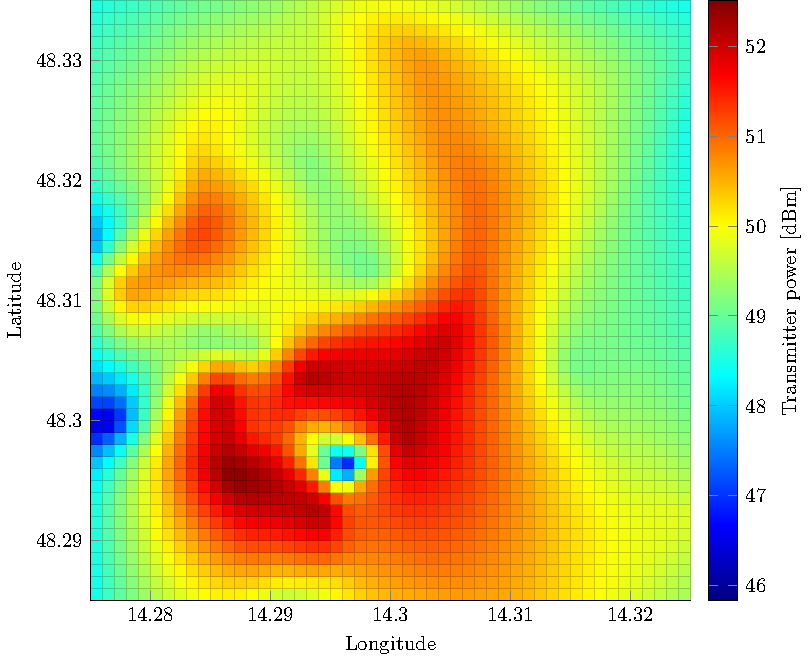
\includegraphics[width=0.9\columnwidth]{senderpower}
	\end{figure}
\paragraph{Modeling the Environment}
The coverage prediction done with the network planning tool needs a model of the real environment in order to predict the coverage area for each BTS. For now the model consist of the location and the transmit power of each BTS. However, as mentioned before the coverage area of the BTS depends also on the landscape characteristics. A representation of the landscape is defined by a digital elevation model that describes the surface. 

The digital elevation model\footnote{The Digital Elevation Model over Europe from the GMES RDA project \url{http://www.eea.europa.eu/data-and-maps/data/eu-dem}} used for the coverage estimation offers a resolution of 25 meters, which means that each pixel covers 25 by 25 meters. During our research we have seen that the resolution of the underlaying elevation model directly affects the quality and, therefore, the accuracy of the coverage prediction.

To improve the coverage prediction further, we integrated a building block model for the two research areas. For the city of Linz, the footprint of every buildings is known from OpenStreetMap\footnote{More information about how building information can be retrieved from OpenStreetMap \url{http://wiki.openstreetmap.org/w/index.php?title=Buildings&oldid=1050850}}, though, their height is unknown. For these buildings we assumed a medium height of 15 meters. On the contrary, the city of Vienna\footnote{The GIS service from the city of Vienna is located here \url{https://www.wien.gv.at/kultur/kulturgut/architektur/gebaeudedaten.html}} provides a building model with height information. The building model of the city of Vienna consists of the footprint of the buildings and a category that specifies its height. The available height categories are: 
\begin{itemize}
	\item 1.6 - 4.5 m
	\item 4.6 - 7.5 m
	\item 7.6 - 9.0 m
	\item 9.1 - 12.0 m
	\item 12.1 - 16.0 m
	\item 16.1 - 21.0 m
	\item 21.1 - 26.0 m
	\item $>$ 26 m
\end{itemize}

In our building model we enriched the building footprint from OpenStreetMap for the city of Vienna with the average height of the specified category.

In total we computed two coverage predictions for each research area. The first uses the transmitter's location, transmitter power and the digital elevation model. The second, enhances the first one by additionally using the building model on top of the elevation model.

We will later discuss the differences and benefits of the three -- \emph{Voronoi}, \emph{Network planning coverage prediction}, \emph{Network planning coverage prediction with buildings} -- cell area estimation methods.\newline

Besides modeling the environment for the coverage area prediction we also need a representation of the environment in which the subscriber is moving. In our case we need additional information to narrow down the user's location. The most important is a model of the road network on which the subscriber moves. Since individuals move on predefined ways, our framework focuses on ways, paths and streets. The road network we are using is obtained from OpenStreetMap and freely available. OpenStreetMap covers almost all ways and additionally provides other information such as the maximum allowed speed which is later used to validate and adapt the velocity estimation.\newline

As of now, the framework knows the road network on which the subscriber can move and the coverage area of the cell sites. However, the location inside the borders of the cell site is still unknown. The location within the cell site is an important figure for estimating the trajectory, in particular its start and end positions. To further enhance the localization of the subscriber within the cell site we are using population density and land use information. This information allows the framework to restrict the subscribers location by defining areas, in which it is unlikely that a subscriber starts or ends his journey. The European Environment Agency (EEA) provides both population density\footnote{Population density disaggregated with Corine land cover 2000 \url{http://www.eea.europa.eu/data-and-maps/data/population-density-disaggregated-with-corine-land-cover-2000-2}} and CORINE land cover\footnote{Corine Land Cover 2006 seamless vector data \url{http://www.eea.europa.eu/data-and-maps/data/clc-2006-vector-data-version-3}} maps. The population density map and the CORINE land cover map both have a spatial resolution of 100 meter. Therefore, each pixel covers 100 by 100 meters. We will later discuss how this information was used to estimate the users start and end positions.

\subsection{Subscriber Mobility Estimation}
In the following section, we will delineate the approach used to estimate the subscribers' mobility. It is based on work which has been presented at the European Modeling Symposium 2013~\cite{Kieslich2013}. Here we will explain how the input dataset, such as subscriber's information, coverage prediction, population and land use information is transformed into subscriber's movement trajectories. In particular, handover updates are used to locate the subscriber and derive its velocity. Since that, we improved the trajectory generation with new coverage predictions and handover point estimations. Additionally we integrated an approach to derive the subscribers’ velocity from handover updates.

The general idea is that we have samples of the subscriber's trajectory. At discrete times we know that the user has entered the coverage area of new cell site due to a handover event. We also know that the user started and ended his journey within the first and the last cell site respectively. Still missing, however, is an estimation of a route that traverses each of the cell sites and a location (handover position) to each of the discrete time points, to derive the subscribers’ velocity.
\subsubsection{Estimating the Subscribers Path}
Each trajectory needs an estimation of the route traveled by the subscriber. All we know, from the subscriber's information provided by the network operator, is a series of handover events that gives a rough representation of the route traveled by the user. The following parts will describe in more detail how the subscribers’ path and velocity can be derived from this information.

The estimation of the subscriber's path is an iterative process that takes the cell area estimation, the road network and the subscriber's information as input variables. The process first estimates the start and end positions of the subscriber and then computes a route between these two points. At the end of the process the velocity of the subscriber will be computed by taking the position and the timestamp of consecutive handovers into account.


\paragraph{The Location of the Subscriber}
Until now the location within the cell coverage is still unknown. However, for estimating the subscribers route a start and end points are required. The start and end points of a trajectory are marked by the call establishment event and the call termination event respectively. Therefore, our approach is predicting the subscribers start and end positions within the extent of the cell where the event originated.

To narrow these boundaries, the system uses geographical input (CORINE
land cover) and socio-statistical maps (population density maps).
By using CORINE land cover data the system can define areas where
it is unlikely that a subscriber will start or end his journey. This step can be
parameterized by giving each of the CLC classes a percentage factor. The
percentage defines how likely it is that a subscriber starts or ends a call in
this class. In this manner the subscribers location can be restricted to a few defined CLC classes such as 	artificial surfaces, urban fabric and industrial, commercial and transport units. 

Our second assumption is that subscribers will more likely start or end
their call in a higher populated area within the cell boundaries. Therefore,
the system uses population density maps in order to better estimate the
start or end position.

An example for our assumption is depicted in Figure \ref{fig:populationgrid}, were an area defined by its border with three different population density areas area illustrated. Based on our assumption the subscriber will be more likely located in the area with 240$[\frac{people}{km^2}]$ than in the ones with 45$[\frac{people}{km^2}]$ and 30$[\frac{people}{km^2}]$. Hence, our framework will use all different population density areas within the border and compute a probability density function. After a population area has been chosen by the random process the subscriber's location will be uniformly located within the border of the population area. This process ensures that subscribers will be located with a higher probability in areas with a higher population density.
	\begin{figure}[h!]
		\label{fig:populationgrid}
		\caption{\csentence{Popualtion grid} The following demonstrates an area with 3 different population densities. Our assumption is that people will more likely start or end their journey in a higher populated area.
		}
		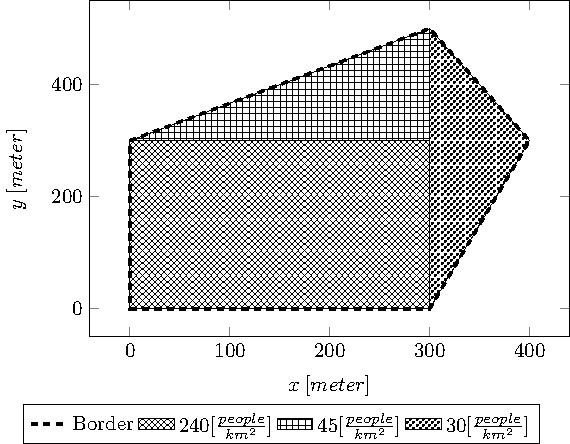
\includegraphics[width=0.9\columnwidth]{populationgrid}
	\end{figure}
%We are using land cover information to restrict the users position within the cell coverage. In this manner we allow the users start and end position to be located in urInstead of a uniform position distribution our approach utilizes a distribution computed from population density maps. This distribution prefers areas with a higher population density within the extent of the cell. Our assumption is that subscribers will most likely start or end their journey in a higher density area than in a less density one.
\paragraph{The Traveled Route}
Since individuals travel most of their time on predefined paths we restrict our generated trajectories to be on top of the road network of the research area. In this manner the subscriber's route will be computed on the OpenStreetMap road network between the before estimated start and end positions. By default, 20 routes with different start and end positions will be computed. Afterwards, these routes will be validated in terms of their geometry and the time it takes to traverse the route.

The first validation calculates the squared sum of the minimum distance between the route and the centroid of each cell areas. This is the same metric that Tettamanti et al.~\cite{Tettamanti2012} used for their system. For each of the previously calculated routes $j$, the squared sum of all minimum distances $d_{i,j}$ between the
route and the cell site was calculated.

We introduce a duration ratio $route_{ratio}$ between the call duration $d_{call}$ and the time it takes to drive the route $d_{route}$ as depicted in Equation~\ref{eq:ratio}. The ratio gives information whether the estimated route is either too fast or too slow. 
\begin{align}
	D_j           & =\sum_{i=1}^{m} \min(d_{i,j})^{2} \label{eq:sumsquaremine} \\
	route_{ratio} & =\frac{d_{call}}{d_{route}} \label{eq:ratio}               
\end{align} 

The squared sum $D_j$ in combination with the duration ratio $route_{ratio}$ was used to chose the most likely route the subscriber has traveled in terms of distance to cell sites and travel time.
\subsubsection{Deriving Velocity from Handover Positions}
To describe the mobility of the subscriber it is important to know its movement over time. In our case the movement is defined by handover events that are issued over time. Whenever a subscriber is in an active call and moves from one cell to another cell, a handover event is issued. This event exposes a coarse location (cell site) and a timestamp. By using this information, the velocity of the subscriber can be derived. The velocity of a subscriber is an important figure for mobility simulation, since the velocity, together with the estimated route, describes the movement of the subscriber. However, as the system only knows the cell in which the handover event originated -- cell to which handover was made -- an estimation of the actual handover point is needed.
\paragraph{Predicting the Handover Position}
The framework uses two consecutive handovers to compute the origin of the handover position. In theory, a handover is carried out whenever a subscriber leaves the coverage area of one cell site and enters the coverage area of another cell site. In practice, however, there are more aspects that affect a handover event, besides the coverage area of a cell site. These aspects can be for instance network load, network interference on the channel, etc.

In our research we focus on the handover prediction based on the coverage of the involved cell sites, since there is no information of the network load or the network interference available in the event stream provided by the network operator.

Throughout our investigation of handover sequences we discovered three different types of handover. The first is defined as an \emph{overlapping handover}. 
An overlapping handover is where the coverage areas of the two involved cell sites have an intersection. Note that an overlapping handover can not occur when using Voronoi diagrams for the cell area estimation since Voronoi diagrams are not overlapping. However, when using a network planning tool for the coverage area estimation there are many cell sites whose coverage areas overlap. 

\begin{figure}[h!]
		\label{fig:handover}
		\caption{\csentence{Types of handover} An overlapping handover (a) and an unconnected handover are depicted together with the estimated handover position (red point)
		}
		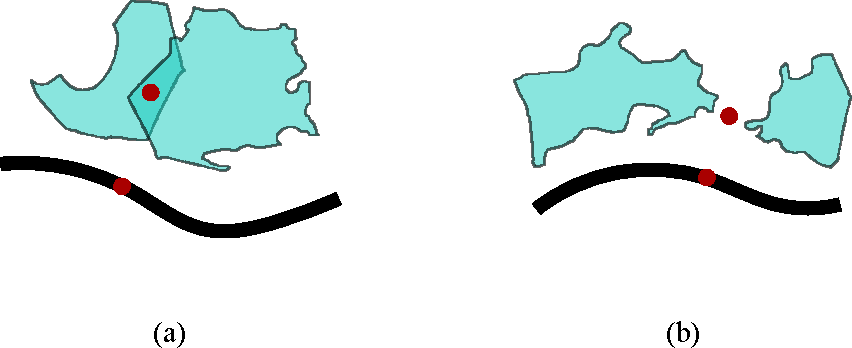
\includegraphics[width=0.9\columnwidth]{handover}
	\end{figure}

The second handover, is an \emph{unconnected handover}, where the involved coverage areas do not intersect. This means that a handover is made to a cell site whose coverage area the subscriber has not entered yet. Figure~\ref{fig:handover} illustrates the differences between an (a) overlapping and (b) an unconnected handover.

The third, ping-pong handover is where a handover is made from cell site $A$ to cell site $B$ and later back to $A$. These handovers are an undesirable effect not only for the network itself but also for the timing estimation. Therefore, we filtered out ping-pong handovers by removing the last handover event, in this case the handover event from $B$ to $A$.

Algorithm \ref{alg:prediction} depicts how the system estimates the handover position for overlapping and unconnected handover. For an overlapping handover the centroid of the intersection $C=A \cap B$ of the involved cell site is computed and then the nearest point on the calculated route is set as the handover position. 

For unconnected handover the line between the closest points of the two coverage areas is computed, if this line intersects the before computed route then the intersection position is set as the handover position. If this is not the case then the midpoint of the line is computed and the nearest point on the calculated route is set as the handover position. The last step in each of these branches was performed to associate the handover position with the road network.
%\SetAlFnt{\footnotesize}
%
%\begin{figure}[!t]
%	\removelatexerror
%	\begin{algorithm}[H]
%		\caption{Handover prediction}
%		\label{alg:prediction}
%		HP$\leftarrow$List()\;
%		\For( \emph{Handover loop}){$i\leftarrow 1$ \KwTo $length(handover)-1$}
%		{
%			curr=handover[i]; next=handover[i+1]\;
%			/*overlapping handover*/\\
%			\uIf{Intersects(curr,next)}{
%				centroid=Centroid(Intersects(curr,next));
%				Add(HP,NearestPoint(route,centroid));
%			}
%			\Else{
%				line=LineBetweenNearestPoint(curr,next)\;
%				/*line crossing route*/ \\
%				\uIf{Intersects(line,route)}{
%					Add(HP,Intersects(line,route))\;
%				}
%				\Else{
%					midPoint=MidPoint(line)\;
%					Add(HP,NearestPoint(route,midPoint))\;
%				}
%			}
%		}
%	\end{algorithm}
%\end{figure}
\begin{figure}
\begin{algorithmic}[1]


 \State $HP\gets List()$
 \For{$i<length(handover)-1$}
 \State $curr=handover[i];next=handover[i-1]$
 
  \EndFor
\If {$Intersects(curr,next)$}
   \State $c=Centroid(Intersects(curr,next))$
   \State $Add(HP,NearestPoint(route,c))$
\Else
	\State $line=LineBetweenNearestPoint(curr,next)$
    \If {$Intersects(line,route)$}
        \State $Add(HP,Intersects(line,route))$
        \Else
        \State $mp=MidPoint(line)$
        \State $Add(HP,NearestPoint(route,mp))$
    \EndIf
\EndIf
\end{algorithmic}
\caption{Euclid's algorithm}\label{alg:prediction}
\end{figure}

\paragraph{Computing the Average Velocity}
To derive the subscriber's mobility and in generally its movement the velocity needs to be computed. 
After the handover positions have been estimated the average velocity of the subscriber between two consecutive handover points can be computed. 
Each of the handover points contains a timestamp, that indicates when the handover event occurred. To derive the velocity, the distance between the two handover points is divided by the time difference of the two timestamps. The distance denotes to the distance on the road network and not to the linear line. 

\paragraph{Velocity Validation}
Due to the deviation between the observed (real) handover position and the estimated handover position, the subscriber's velocity can differ. During the development of the framework we discovered that certain handover can lead to a velocity overrun. Hereby, two handover events were made in a short period of time $t<10$ seconds where the distance between the two handover events is fairly large compared to the small time difference. By computing the velocity between these two handovers the resulting velocity was few times higher than the maximum allowed speed on that particular road. This was affected by a wrong handover position estimation and lead to the development of an adaption algorithm (see Algorithm ~\ref{alg:adaption}) that first validates each velocity and later rearranges the handover position in case the computed velocity was higher than a defined threshold. 

The general approach is that in case of a velocity overrun the algorithm repositions the handover positions between the current and either the predecessor, the successor or both handover events.

The algorithm iterates over the whole trajectory after the velocity for each handover segment has been computed. A handover segment is a part of the route from one handover position to a subsequent handover position and the average velocity of the segment. For each handover segment, the algorithm compares the velocity with the maximum allowed speed of that particular road. In the case the velocity is $1.7$ times higher than the maximum allowed speed, handover repositioning takes place. 

The first step is to calculate the distance the subscriber can drive at the maximum allowed speed for the duration of the handover segment. The duration is defined by the timestamps difference of the involved handover. The difference between the computed allowed distance and the distance between the two handover positions corresponds to the handover position deviation. For the current handover segment the velocity will be set to maximum allowed speed. If the handover segment has no predecessor, but a successor then the difference between the computed allowed distance and the distance between the handovers will be added to the successor. Likewise, if the handover segment has a predecessor but no successor the reposition works the same just the successor is replaced by the predecessor. 

If, however, the handover segment has both a predecessor and a successor, which is the case for most handover segments, then the algorithm repositions either the first handover position, all two handover positions or the second handover position. At first the algorithm is equally adding the difference between the allowed distance and the distance of the handover segment to the predecessor and successor. In the case that the velocity of the predecessor is greater than the maximum allowed speed after repositioning, the reposting of the predecessor will be withdrawn and the repositioning will only affect the successor. In equal measure, this will be done to the successor if its velocity exceeds the maximum allowed speed. 

  

%\SetAlFnt{\footnotesize}
%\begin{figure}[!t]
% \removelatexerror
%  \begin{algorithm}[H]
%   \caption{Handover adaption}
%   \label{alg:adaption}
%   \For( \emph{Adaption loop}){$i\leftarrow 1$ \KwTo $length(trajectory)$}
%   {
%   	allowedSpeed<-MaxSpeed(trajectory[i])\;
%   	c=trajectory[i]\;p=trajectory[i-1]\;n=trajectory[i+1]\;
%      /*speed overrun*/\\
%      \uIf{Speed(c)$\geq1.7$*allowedSpeed}{
%      	cDist=Distance(c)\;
%      	pDist=Distance(p)\;
%      	nDist=Distance(n)\;
%      	nomDist=allowedSpeed*Duration(c)\;
%      	SetSpeed(c,allowedSpeed)\;
%      	\uIf{p==NULL$\&\&$n!=NULL}{
%      		pDist=pDist+(cDist-nomDist)\;
%      		SetSpeed(prev,pDist/Duration(p))\;
%      	}
%      	\uElseIf{p!=NULL$\&\&$p!=NULL}{
%      	nDist=nDist+(cDist-nomDist)\;
%      	SetSpeed(n,nDist/Duration(n))\;
%      	}
%      	\uElse{
%      	      	nTempDist=nDist+(cDist-nomDist)/2\;
%      	      	pTempDist=pDist+(cDist-nomDist)/2\;
%      	      	\uIf{nTempDist/Duration(n)$\gg$nomSpeed}{
%      	      	nTempDist=nDist;
%      	      	pTempDist=pDist+(cDist-nomDist)\;
%      	      	}
%      	      	\uElseIf{pTempDist/Duration(p)$\gg$nomSpeed}{
%      	      	      	      
%      	      	      	      	nTempDist=nDist+(cDist-nomDist)\;
%      	      	      	       	pTempDist=nDist;
%      	      	  }
%      	      	SetSpeed(n,nTempDist/Duration(n))\;
%      	      	SetSpeed(p,pTempDist/Duration(p))\;
%      	}
%      }
%      }
%  \end{algorithm}
%\end{figure}

%\begin{figure}[!t]
%	\removelatexerror
%	\begin{algorithm}[H]
%		\caption{Handover adaption}
%		\label{alg:adaption}
%		\For( \emph{Adaption loop}){$i\leftarrow 1$ \KwTo $length(trajectory)$}
%		{
%			allowedSpeed<-MaxSpeed(trajectory[i])\;
%			c=trajectory[i]\;p=trajectory[i-1]\;n=trajectory[i+1]\;
%			/*speed overrun*/\\
%			\uIf{Speed(c)$\geq1.7$*allowedSpeed}{
%				cDist=Distance(c)\;
%				pDist=Distance(p)\;
%				nDist=Distance(n)\;
%				nominalDist=allowedSpeed*Duration(c)\;
%				SetSpeed(c,allowedSpeed)\;
%				\uIf{p==NULL$\&\&$n!=NULL}{
%					pDist=pDist+(cDist-nominalDist)\;
%					SetSpeed(prev,pDist/Duration(p))\;
%				}
%				\uElseIf{p!=NULL$\&\&$p!=NULL}{
%					nDist=nDist+(cDist-nominalDist)\;
%					SetSpeed(n,nDist/Duration(n))\;
%				}
%				\uElse{
%					nTempDist=nDist+(cDist-nominalDist)/2\;
%					pTempDist=pDist+(cDist-nominalDist)/2\;
%					\uIf{nTempDist/Duration(n)$\gg$nominalSpeed}{
%						nTempDist=nDist;
%						pTempDist=pDist+(cDist-nominalDist)\;
%					}
%					\uElseIf{pTempDist/Duration(p)$\gg$nominalSpeed}{
%						      	      	      	      
%						nTempDist=nDist+(cDist-nominalDist)\;
%						pTempDist=nDist;
%					}
%					SetSpeed(n,nTempDist/Duration(n))\;
%					SetSpeed(p,pTempDist/Duration(p))\;
%				}
%			}
%		}
%	\end{algorithm}
%\end{figure}

%\begin{figure}[!t]
%	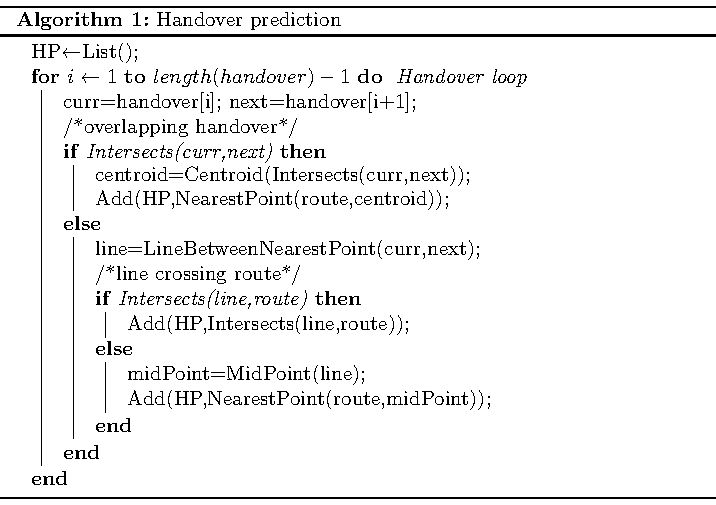
\includegraphics{adaptionalg}
%\end{figure}

\subsection{Evaluation of Subscriber Trajectories}
To evaluate our findings we define a set of measurements that will be computed for each of the generated movement trajectories. To validate the route geometry, the handover position and the velocity of the subscriber we recored a GPS track for each test ride. Additionally we stored the position of each handover by tracking changes in the Cell-Id and LAC on the handset and storing the location when the subscriber is connected to a new cell site. From the GPS track and the timestamp information the velocity of the subscriber can be derived and later be compared with the estimated one. The velocity evaluation compares  the average velocity of the subscriber between two handover points with the estimated velocity. GPS was only used during research in order to validate our approaches and assumption.

For our investigation we generated and evaluated trajectories for mobile network subscriber's for three -- Voronoi diagrams, Network planning tool and Network planning tool with buildings -- different coverage estimation methods.
\subsubsection{Route Geometry}
An important aspect of the trajectory generation process is to identify the route traveled by the network subscriber. In order to evaluate our approach of computing the route between a computed start and end position we used two different metrics. This metrics are the Hausdorff distance and the Fr\'{e}chet distance and were used to compute the similarity between the traveled (GPS) and the estimated route. 

To compute the maximum deviation between the estimated route and the actual subscriber route the Hausdorff distance was computed. The Hausdorff distance is defined as the greatest of all the distances from a point in one set to the closest point in the other set. In our case $X$ and $Y$ are the estimated and the actual route respectively.
\[ d_{H}(X,Y) = \max\{\,\sup_{x \in X} \inf_{y \in Y} d(x,y),\, \sup_{y \in Y} \inf_{x \in X} d(x,y)\,\}\]

The Fr\'{e}chet distance was introduced by Fr\'{e}chet~\cite{Frechet} and is well-suited for the comparison of trajectories since they take the continuity of the trajectory into account. In our evaluation we are using the algorithm by Alt and Godau~\cite{Alt1995} that computes the Fr\'{e}chet distance on two polygonal curves in Euclidean space.

The Fr\'{e}chet distance for two curves $A,B:[0,1]\rightarrow V$, in our case two routes, is defined as 
%\[F(A,B) = \inf_{\alpha, \beta}\,\,\max_{t \in [0,1]} \,\,  \Bigg \{d \Big ( A(\alpha(t)), \, B(\beta(t)) \Big ) \Bigg \}\]


\[\delta_F(f,g)=\inf_{\substack{\alpha [0,1] \rightarrow [a,a'] \\\beta [0,1] \rightarrow [b,b']} }\,\, \max_{t \in [0,1]} \,\, \lVert f(\alpha(t))-g(\beta(t)) \rVert\]
where $\alpha$ and $\beta$ are continuous and increasing functions with $\alpha(0)=a$, $\alpha(1)=a'$, $\beta(0)=b$ and $\beta(1)=b'$. 

Our evaluation was done using Christophe Genolis\footnote{More information about the implementation of the Fr\'{e}chet distance \url{http://www.inside-r.org/packages/cran/longitudinalData/docs/distFrechet}} implementation of the Fr\'{e}chet distance.

\subsubsection{Velocity Comparison}
A trajectory consists of the traveled route as well as timestamps that define when a point on the route has been traversed. This information describes the velocity of the subscriber on the road. In order to evaluate our approach, to estimate the subscriber's velocity based on handover positions, we compare the estimated velocity with the ground truth velocity obtained by the GPS information. Another aspect was to evaluate the performance of the adaption algorithm that repositions handovers in case a velocity overrun happened.

One of the metrics is the mean absolute error (MAE )between the observed average velocity $ Y_i$  and the computed velocity $ \hat{Y_i}$. The observed average velocity $Y_i$ is a subset of the velocity obtained from GPS between the two consecutive handover positions of the researched handover segment. The computed velocity is the velocity derived from computing the distance between the consecutive handover points divided by the timestamp difference. We also used the root mean square error (RMSE), that is stronger influenced by large errors than by small errors.

\[\operatorname{MAE}  = \frac{1}{n}\sum_{i=1}^{n} \left(\lvert \hat{Y_i} - Y_i) \rvert \right)\]
\[\operatorname{RMSE}=\sqrt{\frac{\sum_{i=1}^n (\hat Y_i - Y_i)^2}{n}}\]

Where $n$ is the amount of handover segments for which the velocity was computed with Algorithm~\ref{alg:adaption}.
\subsubsection{Handover Deviation}
Since we estimate the handover position based on the geometry of the coverage area of the involved cell sites we need a metric that indicates how far the estimated handover positions is away from the observed ground truth handover position. The Euclidean distance between the estimated handover position and the observed handover position is used as a metric. This metric is used to evaluate the handover position prediction as well as the coverage area estimation that is used by the handover position prediction algorithm.

\section{Experiments and Results}
\label{sec:results}
After we delineated our approach, for the estimation of movement trajectories for cellular network subscribers', we now present our results and the environment in which they were performed. The here presented results were gathered during four test drives in urban and semi-rural areas in Austria. The first part will introduce the environment in which the test drives were performed and the equipment that was used. The second part presents the gathered results in terms of route geometry, handover deviation and velocity estimation. We will show that is possible to estimate valid and reliable trajectories for cellular subscribers'.

In the tables and figures of this sections we are using the following acronyms to refer to the three coverage estimation methods: P for network planning coverage prediction, PB for Network planning coverage prediction with building models and V for Voronoi diagrams.
\subsection{Environment}
In this section we will present the environment in which the four test drives took place and the information that was captured by handset. For each of the test drives we were using the same handset with the same subscriber identity module (SIM). The handset in use was a Samsung S3 running Android 4.1.1 JellyBean. As mentioned before the handset was used to initiate a call with a second subscriber and maintain the call for the duration of the test ride. During the call the handset stored the location of the subscriber by using GPS and additionally the current connected cell site (Cell-ID and Location Area Code). The network operator later provided subscriber information for each test drive that was consumed by the framework to estimate the trajectories.

Table~\ref{table:tracks} gives an overview of the start and end position and the amount of handover events for each of the four test rides. The amount of handovers in brackets correspond to unfiltered raw events. The one outside are filtered handover where the framework removed ping-pong handover. We  The first test drive started in the city of Linz and ended in the village Treffling that is located in the outskirts of Linz. This test drive was performed entirely on the higher road network and features a semi-rural scenario that consists of an urban and rural part. The second test drive took place within the borders of the city of Linz. The test drive was performed on streets of the minor road network as well as on the city highway. The third and fourth test drive took place within the borders of the city of Vienna. Both test drives were performed on the major and minor road network.

	\begin{table}[h]
		\caption{Overview of the start and end position and the amount of handover events (unfiltered handover) for the four test drive trajectories}
		\begin{tabular}{|c|c|c|c|}
			\hline
			\textbf{$\#$} & \textbf{Start [Lat,Lon]} & \textbf{End [Lat,Lon]} & \textbf{Handover} \\ \hline
			1             & 48.28105,14.30415        & 48.33499,14.3780       & 18 (22)           \\ %563
			2             & 48.31616,14.29052        & 48.28169,14.30275      & 17 (19)           \\  %1058
			3             & 48.13993,16.32367        & 48.19880,16.25597      & 16 (20)           \\ %367
			4             & 48.19283,16.27260        & 48.15278,16.30172      & 27 (37)           \\  \hline %144
		\end{tabular}
		\label{table:tracks}
	\end{table}

In Figure~\ref{fig:563} and \ref{fig:144} the first and the fourth trajectories are illustrated. Each of the three coverage prediction methods -- Network planning tool (a), Network planning tool with buildings (b) and Voronoi diagrams (c) -- along with the estimated handover position is depicted. The last Figure (d) shows the route of the test drive with the exact location of each handover. Due to the limited place the second and third trajectory was omitted.

	\begin{figure*}[h!]
		\label{fig:563}
		\caption{\csentence{Trajectoy 1} A comparison of handover deviations between the real handover position and the estimated one with the three coverage estimation methods (P coverage prediction, PB coverage prediction with buildings and V Voronoi)
		}
		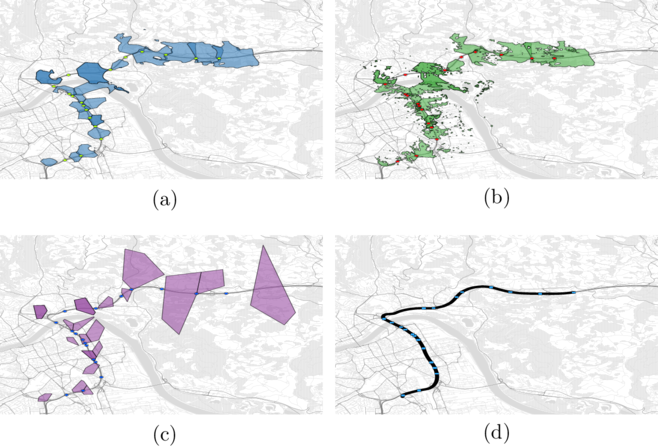
\includegraphics[height=0.40\textheight]{images/563standalone.png}
	\end{figure*}
	
	
	
	\begin{figure*}[h!]
		\label{fig:144}
		\caption{\csentence{Trajectory 4} A comparison of handover deviations between the real handover position and the estimated one with the three coverage estimation methods (P coverage prediction, PB coverage prediction with buildings and V Voronoi)
		}
		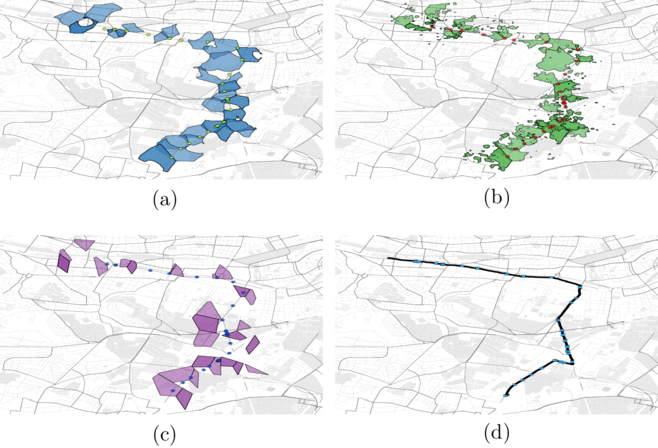
\includegraphics[height=0.40\textheight]{images/144standalone.png}
	\end{figure*}

\subsection{Results}
After introducing the environment in which we performed our test drives, we will now present the results gathered during the test drives. We divided the results into three categories --\emph{route geometry}, \emph{handover deviation} and \emph{velocity estimation} -- that will be delineated in the following sections. The results indicate that the subscriber's route, the handover position and the velocity can be estimated for the purpose of mobility simulations.
\subsubsection{Route Geometry}
To validate the similarity of the estimated route and the actual route the before mentioned discrete Hausdorff distance and the Fr\'{e}chet distance were used. While the Fr\'{e}chet distance is better suited for curve matching the Hausdorff distance gives us the maximum distance between the estimated and the actual route. Hereby, the Hausdorff either indicates the maximum distance between the estimated start and end positions or the maximum distance between the estimated and the actual route. The results in Table~\ref{table:routesim} show a minimum and maximum Hausdorff distance of $0.0075^\circ$ (590m) and $0.0151^\circ$ (1189m) respectively. The minimum and maximum Fr\'{e}chet distance of $0.0012^\circ$ (94m) and $0.0047^\circ$ (370m) respectively. Hence, all the estimated trajectories show a high similarity with the actual route and are therefore suited to describe the subscriber's mobility.

	\begin{table}[h]
		\caption{The route similarity computed with the discrete Hausdorff distance and the Fr\'{e}chet distance}
		\begin{tabular}{|c|c|c|}
			\hline
			\textbf{Trajectory} & \textbf{$d_{H}(X,Y)$ } & \textbf{$\delta_F(f,g)$} \\ \hline
			1                   & $0.0135^\circ$         & $0.0047^\circ$           \\ %563
			2                   & $0.0075^\circ$         & $0.0015^\circ$           \\  %1058
			3                   & $0.0151^\circ$         & $0.0021^\circ$           \\ %367
			4                   & $0.0107^\circ$         & $0.0012^\circ$           \\  \hline %144
		\end{tabular}
		\label{table:routesim}
	\end{table}
\subsubsection{Handover Deviation}
The accuracy of velocity estimation directly depends on the handover estimation. Therefore, it is important to validate the handover position algorithm. We compared the handover positions estimated with the three coverage prediction method against the real handover position stored by the handset. Though Voronoi diagrams only takes the location of the cell sites into account, the handover position could be estimated reasonably well. We saw that Voronoi diagrams worked best in urban areas where the density of cell sites is high. In rural areas, with less cell sites, the Voronoi diagrams became fairly large since the extent is only limited by the surrounding cell sites. 

In Figure~\ref{fig:handoverdeviation} the handover deviation for the first trajectory is illustrated for each handover position. It can be seen that the deviation error increased in the second half of the plot. This was caused by leaving the urban area and driving into a suburban one. Here, Voronoi diagrams performed worse compared to the other coverage predictions.

\begin{figure}[h!]
		\label{fig:handoverdeviation}
		\caption{\csentence{Trajectory 1 handover deviations} A comparison of handover deviations between the real handover position and the estimated one with the three coverage estimation methods (P coverage prediction, PB coverage prediction with buildings and V Voronoi)
		}
		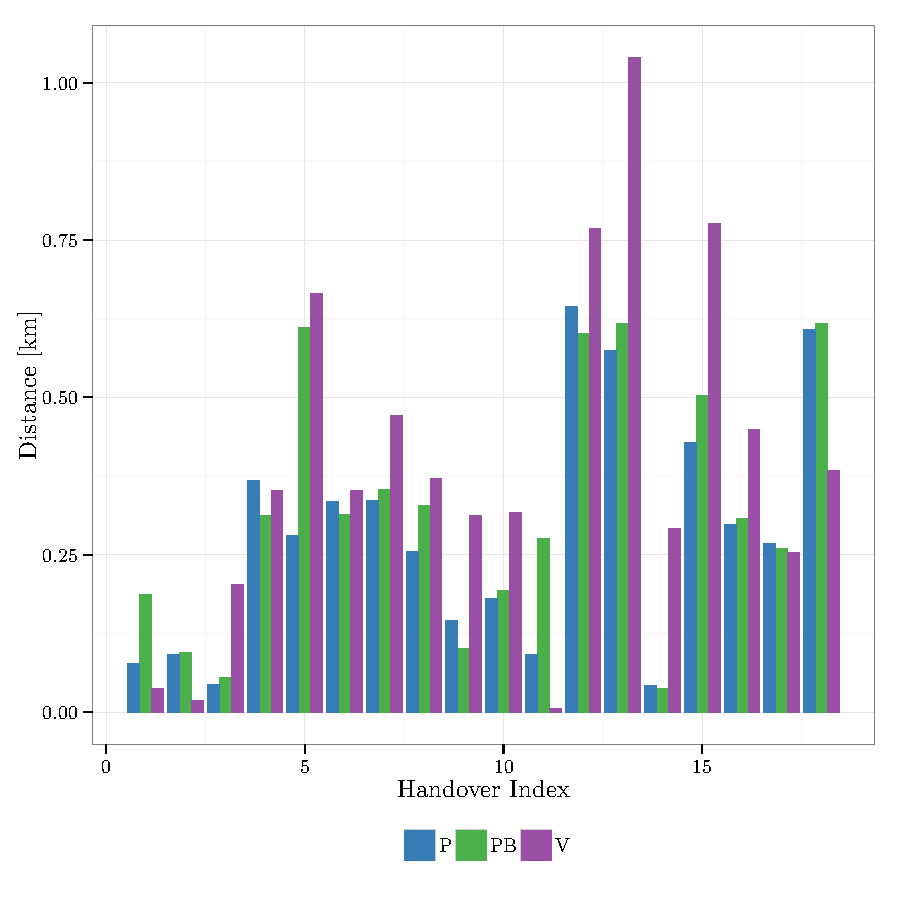
\includegraphics[width=0.9\columnwidth]{images/563_HandoverDeviation}
\end{figure}

Table~\ref{table:handover} gives a statistical overview of the handover deviation between the estimated position and the observed one. All handover positions have been estimated with Algorithm~\ref{alg:prediction} and were performed with the three coverage prediction methods. 
	\begin{table}[h]
		\caption{The min, first quartile, median, mean, third quartile and max handover position deviation in kilometer for each of the four trajectories for the three different coverage predictions M (P coverage prediction, PB coverage prediction with buildings and V Voronoi)}
		\begin{tabular}{|c|c|c|c|c|c|c|c|}
			\hline
			\textbf{$\#$} & \textbf{M} & \textbf{$\min$} & \textbf{$Q_1$} & \textbf{$\tilde{x}$} & \textbf{$\bar{x}$} & \textbf{$Q_3$} & \textbf{$\max$} \\ \hline
			1             & P          & 0.161           & 0.468          & 0.663                & 0.705              & 0.878          & 1.403           \\ \hline
			1             & PB         & 0.101           & 0.547          & 0.716                & 0.711              & 0.928          & 1.315           \\ \hline
			1             & V          & 0.142           & 0.420          & 0.837                & 0.715              & 1.023          & 1.155           \\ \hline
			2             & P          & 0.219           & 0.286          & 0.321                & 0.401              & 0.483          & 0.900           \\ \hline
			2             & PB         & 0.132           & 0.261          & 0.346                & 0.399              & 0.525          & 0.884           \\ \hline
			2             & V          & 0.048           & 0.229          & 0.343                & 0.386              & 0.482          & 0.900           \\ \hline
			3             & P          & 0.111           & 0.360          & 0.449                & 0.677              & 0.604          & 3.786           \\ \hline
			3             & PB         & 0.148           & 0.338          & 0.451                & 0.679              & 0.536          & 4.062           \\ \hline
			3             & V          & 0.013           & 0.281          & 0.409                & 0.669              & 0.639          & 4.085           \\ \hline
			4             & P          & 0.020           & 0.223          & 0.309                & 0.355              & 0.504          & 0.863           \\ \hline
			4             & PB         & 0.030           & 0.213          & 0.325                & 0.359              & 0.506          & 0.850           \\ \hline
			4             & V          & 0.010           & 0.175          & 0.321                & 0.328              & 0.443          & 0.802           \\ \hline
		\end{tabular}
		\label{table:handover}
	\end{table}
By combining the handover deviations over all four trajectories and computing the MAE and RMSE, the coverage predictions without buildings performed best with a MAE of $0.176$km and RMSE $0.231$km. Followed by the coverage prediction with buildings MAE $0.189$km and RMSE $0.253$km and the Voronoi diagrams with MAE $0.238$km and RMSE $0.311$km.

For the fourth trajectory the minimum, maximum and mean handover deviation was $0.010$km, $0.802$km and $0.328$km respectively which shows that the handover position can be estimated with high accuracy.

The third trajectory shows a high maximum handover deviation that was caused by network that was not performing a handover while driving for 3.55km within the city of Vienna. Since the handover algorithm computed a handover position between the two cell site coverage areas, that were far-off, a large handover deviation occurred.
%predP 0.176
%predPB 0.189
%voronoi 0.238
\subsubsection{Velocity Estimation}
In this section we want to discuss the results of the raw velocity estimation and the adapted velocity estimation with handover repositioning. We compared each of the velocities against the velocity derived from the GPS information. Since the estimated velocity accords to the average velocity between two handover position we computed the average GPS velocity between this two handover points. In Figure~\ref{fig:velocity} the raw estimated velocity for the first trajectory is illustrated. It can be seen that there occur many velocity overruns for eacht of the 3 coverage estimation methods. By comparing this Figure with the handover deviation (see Figure~\ref{fig:handoverdeviation}) it is clear that a velocity overrun happens when a large ($\ge0.5$km) happens. Contrary Figure~\ref{fig:velocityadaption} shows the estimated velocity with adaption and handover repositioning. Hence, we see that the peaks could be reduced. To validate the accuracy, the MAE and RMSE for both velocity estimations for each trajectory and each coverage prediction methods was computed. The results depict in Table~\ref{table:results} show that the adaption algorithm can reduce the error introduce by a wrong handover position estimation.

	\begin{figure}[h!]
		\label{fig:velocity}
		\caption{\csentence{Trajectory 1 velocity without adaption} The estimated velocity for all three coverage estimation methods (P coverage prediction, PB coverage prediction with buildings and V Voronoi) without the adaption algorithm
		}
		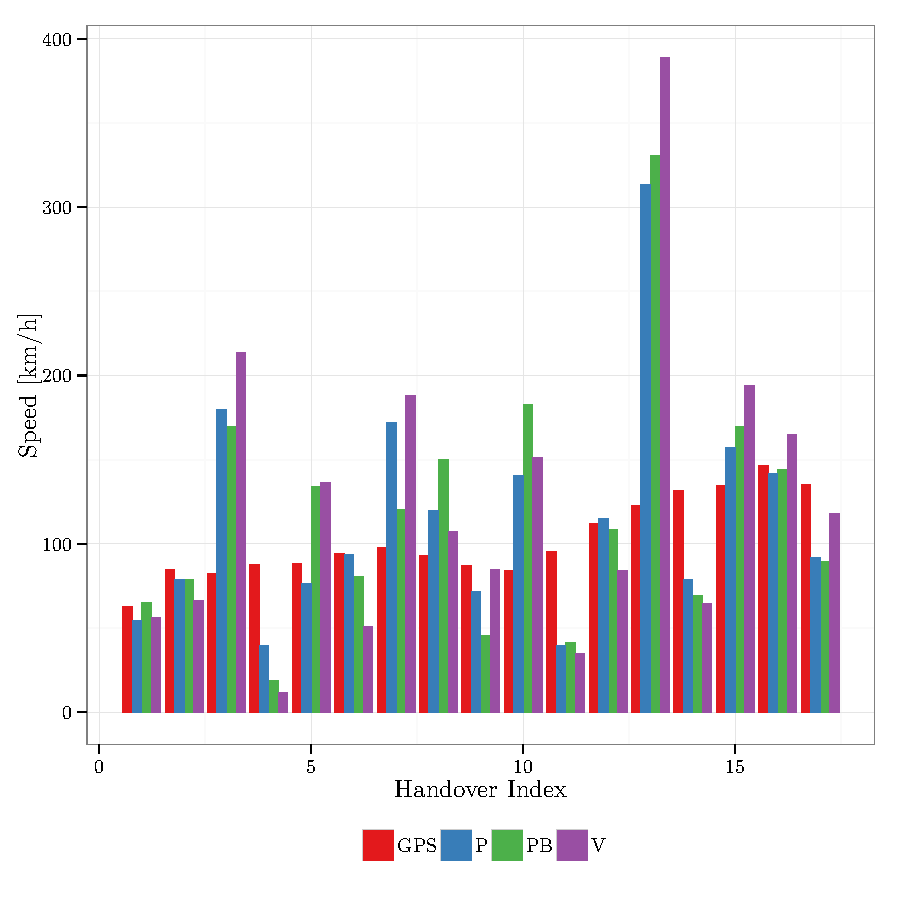
\includegraphics[width=0.9\columnwidth]{images/563_SpeedWithoutAdaption}
	\end{figure}

For the coverage prediction without buildings the velocity MAE, by using the adaption algorithm, was reduced on each trajectory by an average of $60.40\%$. For the coverage prediction with buildings the reduction was $65.75\%$ and for Voronoi diagrams $73.01\%$. 
\begin{figure}[h!]
		\label{fig:velocityadaption}
		\caption{\csentence{Trajectory 1 Velocity with adaption} The estimated velocity for all three coverage estimation methods (P coverage prediction, PB coverage prediction with buildings and V Voronoi) with the adaption algorithm
		}
		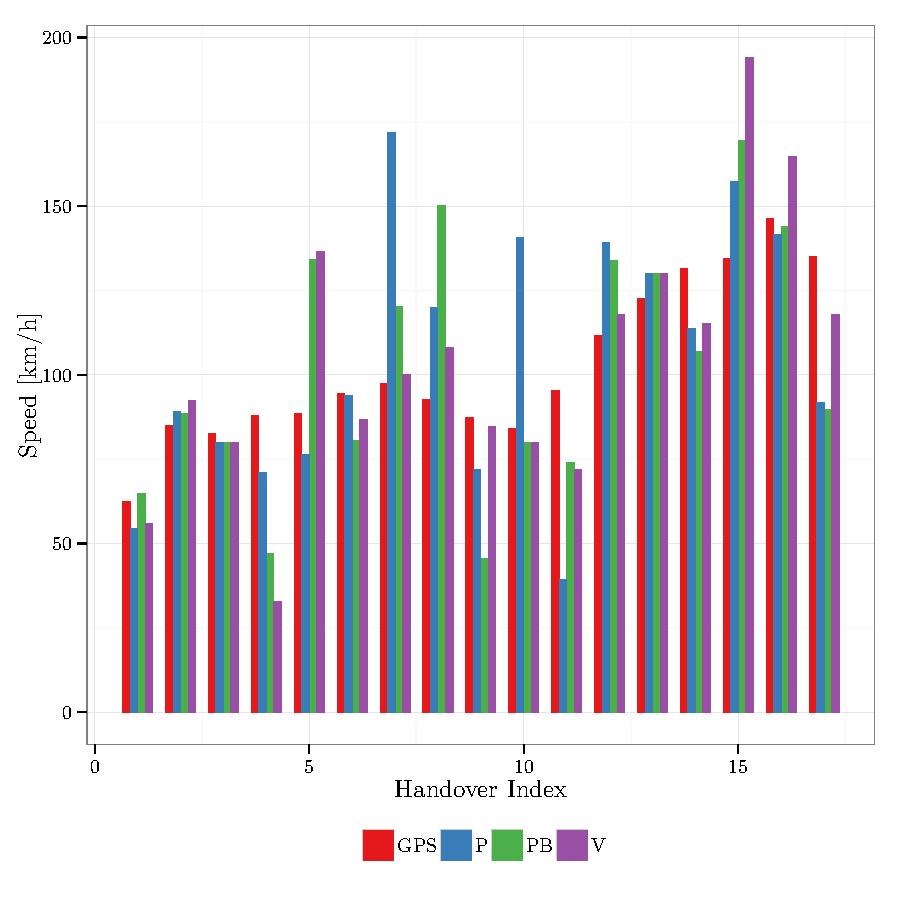
\includegraphics[width=0.9\columnwidth]{images/563_SpeedsWithAdaption}
	\end{figure}
However, this indicates only how well the adaption algorithm work but not how accurate the velocity estimation is in general. To validate the velocity accuracy for the three different coverage prediction methods the absolute adapted velocity errors from the four trajectories were combined to compute the MAE. Here the coverage prediction with buildings had the minimum absolute error for all trajectories with $14.887$km/h. Followed by the Voronoi diagrams with $14.921$km/h and the coverage prediction without buildings $16.004$km/h. 

This indicates that post-processing in the form of the adaption algorithm (Algorithm~\ref{alg:adaption}) is necessary to estimate an accurate velocity. 
	\begin{table}[h]
		\caption{The MAE and RMSE for each of the four trajectories for the three different coverage predictions}
		\begin{tabular}{|c|c|c|c|c|c|}
			\hline
			\textbf{$\#$} & \textbf{M} & \textbf{MAE} & \textbf{RMSE} & \textbf{adaptMAE} & \textbf{adaptRMSE} \\ \hline
			1             & P          & 42.365       & 62.593        & 23.360            & 31.514             \\  \hline %563
			1             & PB         & 50.315       & 69.985        & 23.127            & 29.142             \\  \hline  %1058
			1             & V          & 59.704       & 85.549        & 17.648            & 25.250             \\  \hline%367
			2             & P          & 81.304       & 138.707       & 8.970             & 16.047             \\ \hline %563
			2             & PB         & 60.964       & 99.090        & 9.436             & 12.086             \\   \hline%1058
			2             & V          & 113.999      & 181.854       & 13.029            & 16.932             \\  \hline %367
			3             & P          & 21.125       & 26.808        & 13.305            & 17.799             \\   \hline%563
			3             & PB         & 26.384       & 33.786        & 11.941            & 16.607             \\   \hline%1058
			3             & V          & 28.449       & 40.088        & 13.036            & 18.781             \\  \hline%367
			4             & P          & 58.425       & 150.199       & 17.081            & 22.000             \\  \hline%563
			4             & PB         & 48.061       & 125.747       & 14.553            & 17.795             \\   \hline%1058
			4             & V          & 72.715       & 191.037       & 15.388            & 21.599             \\  \hline %144
		\end{tabular}
		\label{table:results}
	\end{table}

\section{Conclusion and Discussion}
We have shown that trajectories can be estimated for cellular subscribers' by using subscriber information captured in the core network and the location of cell sites. We presented two methods for the cell site coverage estimation and compared them in terms of handover position and velocity estimation. Our results showed that the handover position can be estimated with a mean deviation of 179m by using the coverage prediction without buildings. To minimize the effect of a deviated handover position we developed an adaption algorithm that can reduce velocity overruns and decrease the mean absolute error. The validation has shown that the adaption algorithm reduces velocity overruns at all four test drive trajectories. The mean absolute velocity error over all four trajectory was $14.887$km/h when using coverage prediction with building models. This indicates that the velocity can be precisely estimated for urban and rural areas.

The presented results have shown that cellular network subscriber trajectories can be generated for the purpose of mobility simulations. These trajectories cover the subscriber's route and in addition provide its velocity and are therefore well-suited to describe the subscribers' mobility. %They are well-suited to describe the subscribers' mobility since they cover the traveled route and the velocity.

A future enhancement would be to create a better model of the mobile network to enhance the coverage prediction. This can be achieved by integrating accurate transmitter power and antenna characteristics provided by the networks operator.
